%----------------------------------------------------------------------------------------
%	TITLE OF THE HOMEWORK	
%----------------------------------------------------------------------------------------
{\setlength{\parindent}{0pt}
\title{file title} % Article title
\fancyhead[C]{}
\begin{minipage}{0.295\textwidth} % Left side of title section
\raggedright
CI+CC\\ % Your lecture or course
\footnotesize % Authors text size
%\hfill\\ % Uncomment if right minipage has more lines
Victoria Castor Villegas % Your name, your matriculation number
\medskip\hrule
\end{minipage}
\begin{minipage}{0.4\textwidth} % Center of title section
\centering 
\large % Title text size
Hypothetical Energy Curve\\ % Assignment title and number
\normalsize % Subtitle text size
of dimer Mg-Ne\\ % Assignment subtitle
\end{minipage}
\begin{minipage}{0.295\textwidth} % Right side of title section
\raggedleft
\today\\ % Date
\footnotesize % Email text size
%\hfill\\ % Uncomment if left minipage has more lines
victoria.castor@estudiante.uam.es % Your email
\medskip\hrule
\end{minipage}
}
%----------------------------------------------------------------------------------------
%	HOMEWORK CONTENTS
%----------------------------------------------------------------------------------------


In this work was computed the hypothetical energy curve of Alkaline-Earth
$\cdots$ Rare-Gas dimer: MgNe. All the calculations of the curve were carried
out using the package {\sc{Gaussian16}}~\cite{g16}. The levels of theory
explored was: $i)$ HF-SCF, $ii)$ CI-SD and $iii)$ CC-SD. All our visualization
results was carried out with the help of
{\sc{Matplotlib}}~\cite{Hunter2007} library.

\section{\textbf{Energy Curve at Sapporo-DZP}}

For this first part of the work we use the Sapporo-DZP basis set, which was taken from the
literature \cite{basis_set, Pritchard2019}. Just adding  the basis set at the last part of the
{\sc{Gaussian16}} input. In the input file were also used the \texttt{opt=modredundant}
{\sc{Gaussian16}} keyword to scan around the dimer bond.

As we can expect by Chemical Intuition the Energy Curve does not have an
evident minimum, since the dimer is compounded by Ne which is a Noble Gas and an
Alkaline-Earth metal, Mg. Where Ne basically does not make bonds with another
atoms. Also we can see how the energy increase in way the distance between the
atoms decrease, having accuracy in where the curves starts to go with a higher
slope, \textit{i. e.}, the derivatives of the curves would be similar at every
method studied.

By the other hand the three methods goes to different values when we look at
the energy for long distances. CI-SD and CC-SD goes more similar between
itself than HF with them. HF predict more energy, once again as we expected,
since HF does not take account the correlation energy.

%\begin{figure}[h]%{r}{0.52\textwidth}%{40mm}
\begin{wrapfigure}{r}{0.52\textwidth}%{r}{0.52\textwidth}%{40mm}
\centering
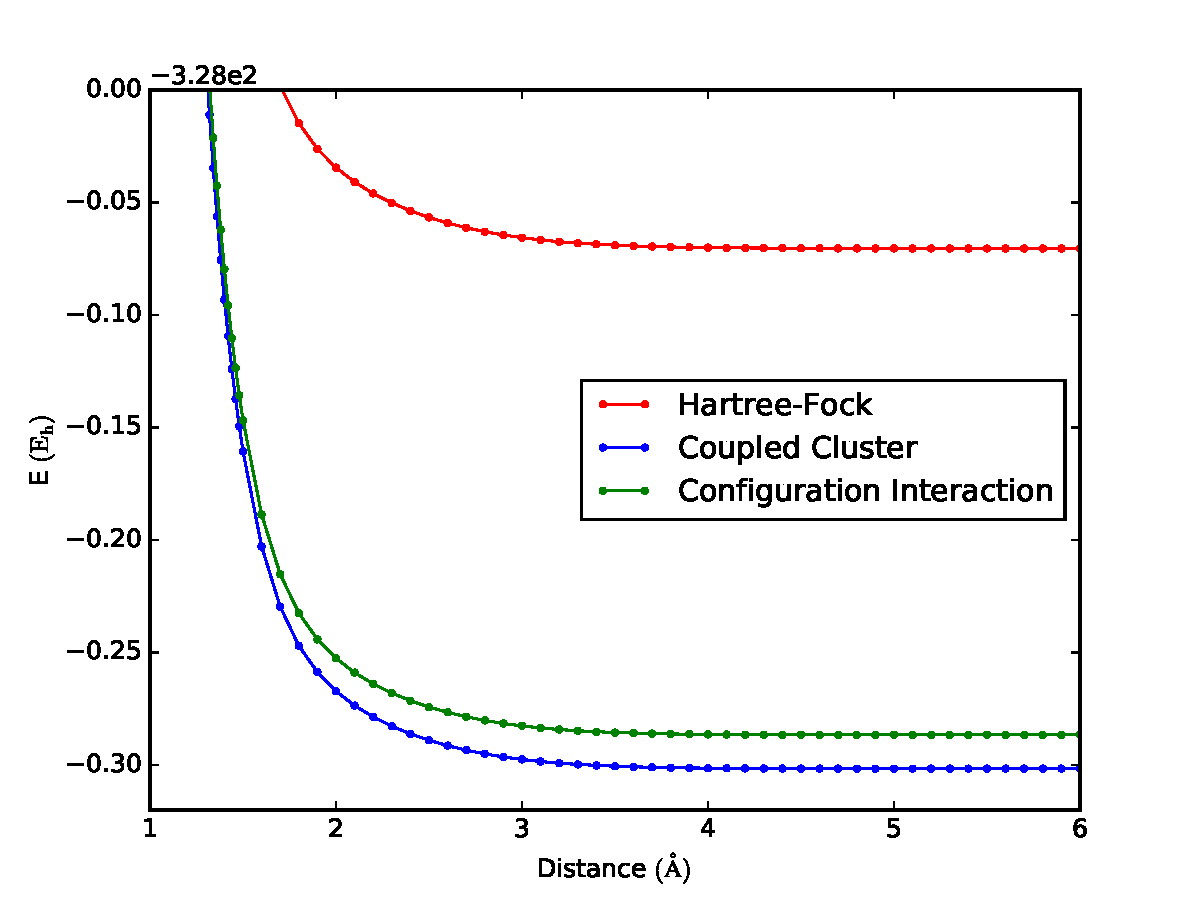
\includegraphics[width=0.52\textwidth]{./img/plots/dzp}%[width=0.1\textwidth]{./img/plots/raw_dzp.pdf}
\caption{Energy curve at Sapporo-DZP}
\label{raw_curve}
\end{wrapfigure}

In Figure \ref{raw_curve} are plotted the Energy Curves. To know the minimum for
every case was necessary analyze numerically the values, that because the
differences are at $10^{-6} \, E\mathrm{_h}$ magnitude order, something that with a naked eye
is impossible to detect that in the same scale as we plot the whole curve (even if we just
look around the minimum is not easy).

The distance values analyzed in this work comes from 0.5 $\AA$ to 1.5 $\AA$ every
0.02 $\AA$, then until 6.5 $\AA$ every 0.1 $\AA$, every 1.0 $\AA$ until
56.5 $\AA$, and finally a last calculation at 100.0 $\AA$, all values are
presented in Supplementary Information \ref{toomuchinformaiton}.
%The
%equilibrium distances found ir for the system at HF, CISD and CCSD level of
%theory are: 5.8, 5.0 and 4.9 $\AA$, respectivily (see Table \ref{data}).

Analyzing the energy values of the curve we found the dissociation energy (Table
\ref{data}).The HF level is nearly one magnitude order distanced of CC-SD and
CI-SD levels, and these ones are more closer between itself.

\begin{table}[b]
\caption{Energy of the system at different theory level, same basis set (Sapporo-DZP)}
\begin{tcolorbox}[tab2,tabularx={X||Y|Y|Y|Y},title=Distance Table,boxrule=0.5pt]
Theory Level    & Eq. distance ($\AA$) & Eq. energy ($\mathrm{kcal/mol}$) & dissociate energy ($\mathrm{kcal/mol}$) & freq. ($\mathrm{cm}^{-1})$ \\\hline\hline
HF              & 5.80                 & -205864.2003          & 0.000987685                 & 2.84                      \\\hline
CC-SD           & 4.90                 & -206009.2676          & 0.016704050                 & 10.20                     \\\hline
CI-SD           & 5.00                 & -205999.8668          & 0.014564275                 & 8.82                      \\
\end{tcolorbox}
\label{data}
\end{table}

\section{\textbf{Frequency}}

Once we know the minimum of the system for the three levels of theory,
the harmonic frequency was computed. As we can see in the Table \ref{data}, for the three methods
the frequency has more or less the same magnitude order, frequency has more
accuracy between methods than energy. Whereas we can see again how CC-SD and
CI-SD have similar value between each other than with HF.

Knowing that the frequency is quantized, since is modeling by the
quantum harmonic oscillator, where for each normal coordinate are given by:

$$
E_n = \hbar\omega\left( n +\frac12 \right) = \hbar\left(n + \frac12 \right) \sqrt{\frac{k}{\mu}} =
hc\left( n +\frac12 \right)\tilde{\nu}
$$

However, we know that the last equation is just in the harmonic case using
as approximation the Hooke Law. In some where the molecule would be at
the dissociation energy. Then, knowing the dissociation energy, the minimum
and how compute the normal coordinate, is just necessary get all
together with the $\tilde{\nu}$ already computed.

\begin{align*}
\Delta E &= hc\tilde{\nu} \left(n_f +\frac12\right) - hc\tilde{\nu} \left(n_i +\frac12\right) \\\nonumber
\Delta E &= hc\tilde{\nu} (\Delta n) \nonumber
\end{align*}

\noindent therefore, with an initial $n$ equals to zero: $n=\Delta E(hc\tilde{\nu})^{-1}$.

For all three cases we have a dissociation energy really small, so small
to no get an $n$ as Natural Number bigger than zero, \textit{i. e.,}
the molecule will never vibrate, since the energy necessary for that
is bigger than the dissociation energy.

\section{\textbf{Bigger Basis Set}}

To get more knowledge in these study was decided study the Sapporo-TZP basis
set, recomputing all values  with Sapporo-TZP, looking for particularly the
minimum value. Specially to know if at the same method with different basis
set gives the same minimum, or how the minimum change.

We summarized on the Table \ref{tab_bigger} how the system accurate with
Sapporo-TZP. We can see that the equilibrium distance change: 0.30, 0.40 and
0.30 $\AA$, comparing with Sapporo-DZP. However, since we are at more than 5.00
$\AA$ these change are not really significant. Whereas the equilibrium energy
does change, around 36, and 75 $\mathrm{kcal/mol}$ for HF and CC-SD/CI-SD
respectively.

Nevertheless, in chemistry we are more interested on the energy differences,
as the dissociate energy. We can see that CC-SD ones again
has the higher dissociate energy. However, all changes in dissociate energy are
under the 0.1 $\mathrm{kcal/mol}$, not meaning a significant difference with
respect the previous calculation.

Also we can see HF is again the higher equilibrium energy and lower dissociate
energy. And how CC-SD and CI-SD are more in a agreement between each other than
HF for equilibrium distance, equilibrium energy and dissociate energy.

Additionally we compute some curves for Sapporo-QZP, the curves are shown on
the Figure \ref{Bigger_theBetter}. For HF theory level the fact that use Sapporo-TZP than
Sapporo-DZP has a significant difference, but not too much comparing Sapporo-TZP with -QTP.
For CI-SD still has an improvement using Sapporo-TZP than -DZP and also
from Sapporo-TZP to -QZP. For CC-SD we have an improvement as in
CI-SD. 

Knowing that the computing time increase using bigger basis set. We aim that
Sapporo-TZP is enough to have a good energies values. Also, because some programs
as {\sc{Gaussian16}} has troubles with
Sapporo-QTP, being necessary use
the next keywords: \texttt{integral=NoXCTest integral=grid=ultrafine}.


\begin{table}[b]
\caption{Energy of the system at different theory level, same basis set (Sapporo-TZP)}
\begin{tcolorbox}[tab2,tabularx={X||Y|Y|Y|Y},title=Distance Table,boxrule=0.5pt]
Theory Level    & Eq. distance ($\AA$) & Eq. energy (kcal/mol) & dissociate energy (kcal/mol)  \\\hline\hline
HF              & 6.10                 & -205900.7260          & 0.004666090                  \\\hline
CC-SD           & 5.30                 & -206085.0827          & 0.021378925                  \\\hline
CI-SD           & 5.30                 & -206075.7918          & 0.019345825                  \\
\end{tcolorbox}
\label{tab_bigger}
\end{table}

Moreover, with all of these values already computed we can calculate the limit of the basis set, at CC-SD
and CI-SD for the $E_\mathrm{corr}$. The behavior of the limit is shown in
Figure \ref{Ecorr}. Since we know that we compute the limits as:

$$
E_{limit} \approx \frac{E_X -bE_{X-1}}{1-b}, with:\  b=e^{B}=\frac{E_X - E_{X-1}}{E_{X-1}-E_{X-2}}
$$

\noindent but also we can get a good approach with two points, computing:

$$
E_{limit} = \frac{E_X X^3 - E_Y Y^3}{X^3 - Y^3},
$$

\noindent where $X$ and $Y$ are the type of bases that we are in.

\begin{figure}%{0.40\textwidth}
    \centering
    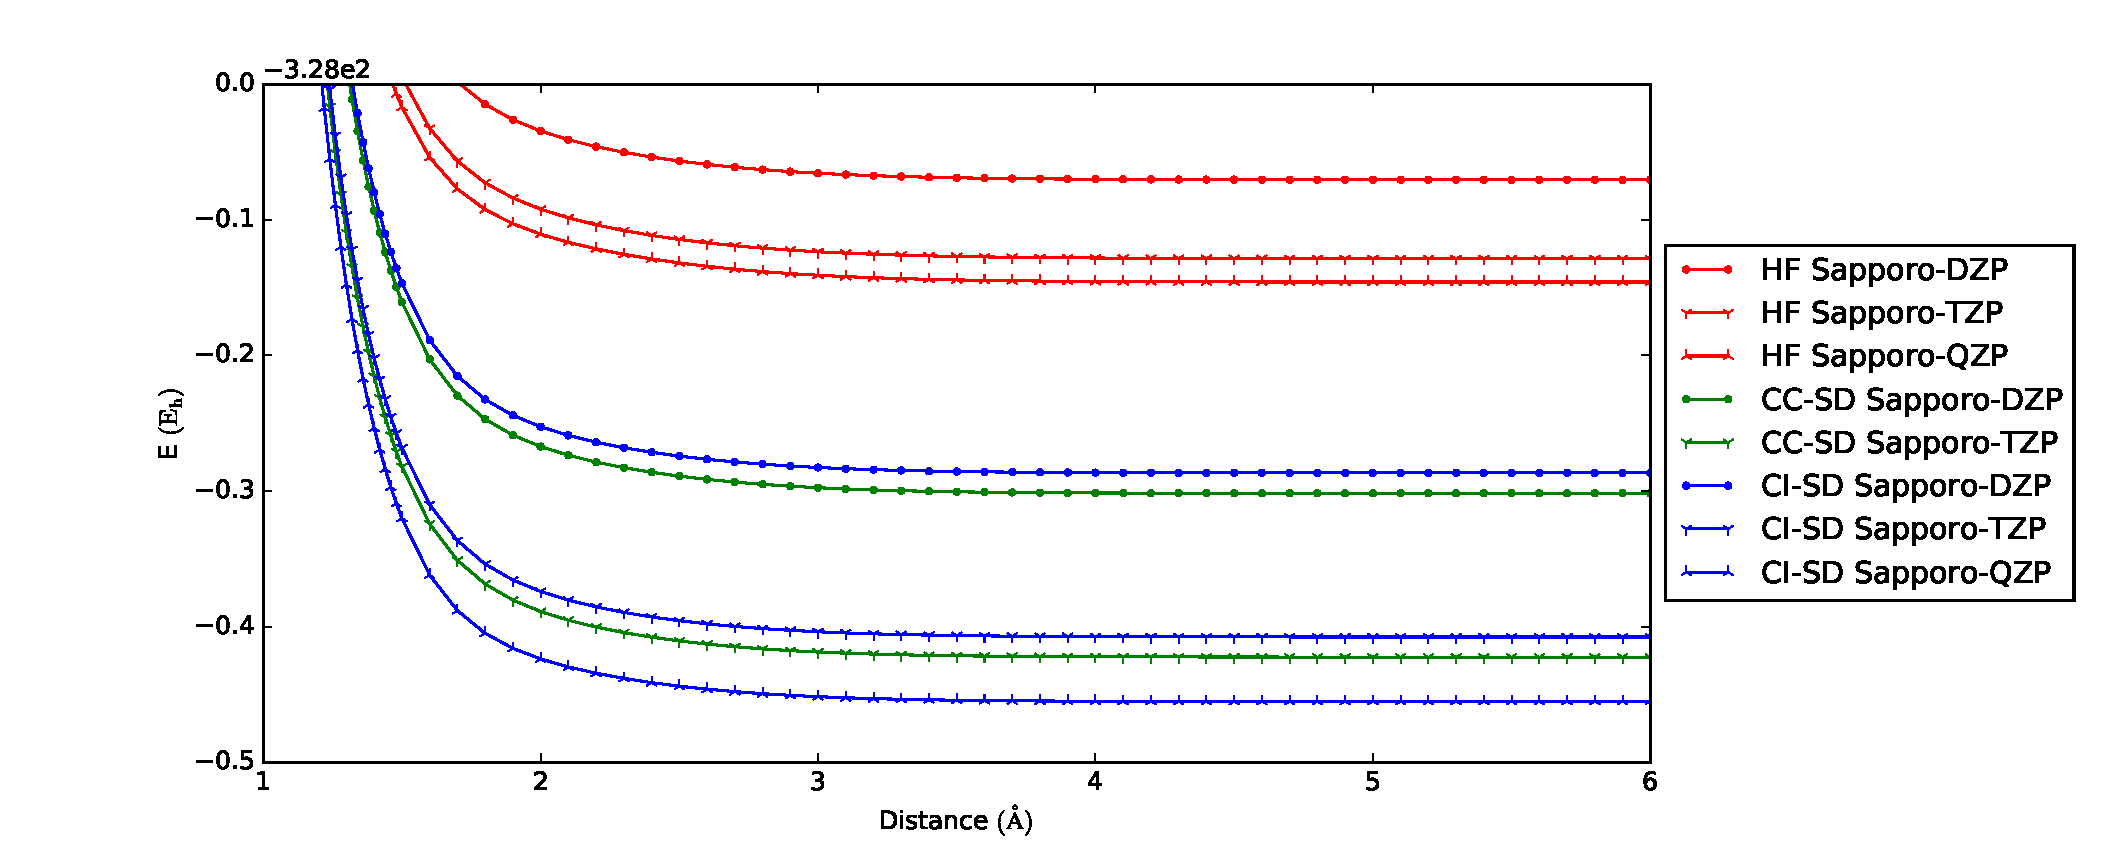
\includegraphics[width=0.95\textwidth]{./img/plots/vs_dt_hfcicc_q_.pdf}
    \caption{Energy curve at different methods with Sapporo D-, T- \& Q-ZP basis set.}
\label{Bigger_theBetter}
\end{figure}

\begin{figure}%{0.40\textwidth}
    \centering
    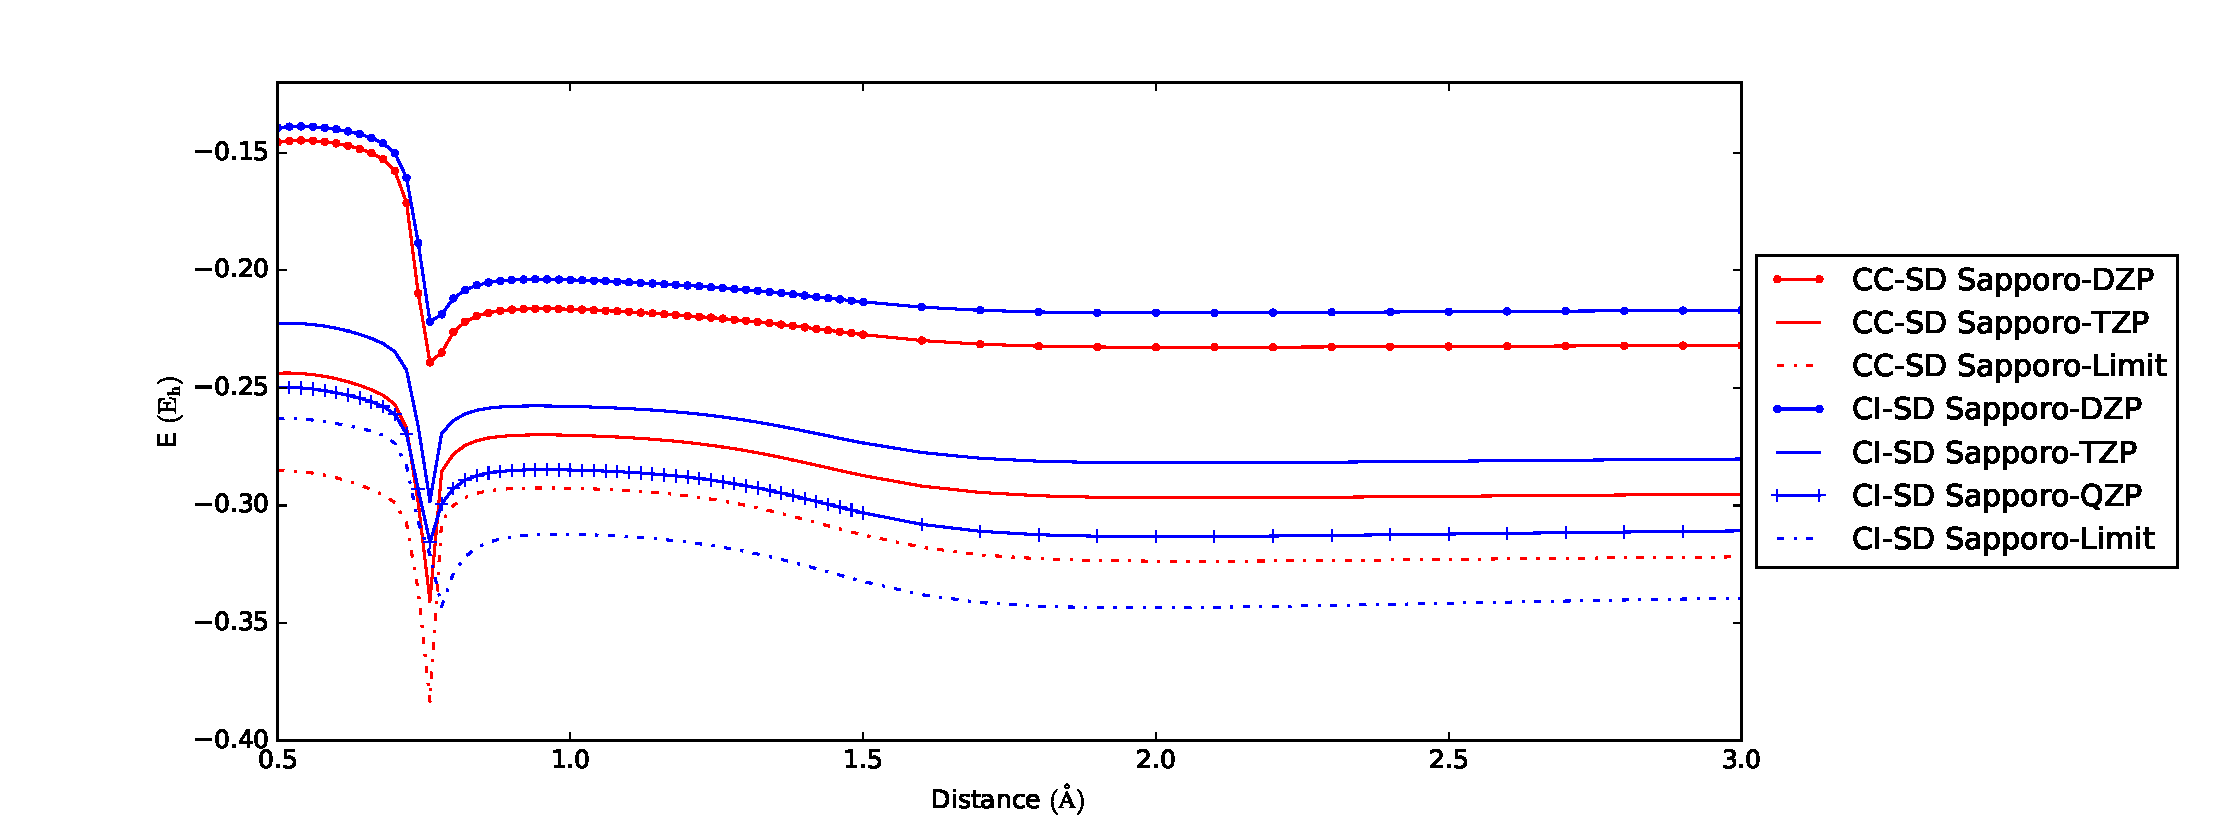
\includegraphics[width=0.95\textwidth]{./img/plots/basis_limit_.pdf}
    \caption{Energy curve for $E\mathrm{_{corr}}$ with limit of Sapporo Basis Set.}
\label{Ecorr}
\end{figure}

\newpage

As we can see in Figure \ref{Ecorr}, for both cases CC- \& CI-SD the $E_{\mathrm{corr}}$ has the same
accuracy. The system has a peak around 0.75 $\AA$, where the system has more
$E_{\mathrm{corr}}$. That peak has no importance for the final
curve, since around 0.75 $\AA$ the repulsion energy is larger enough to be
the head contribution. Finally the $E_{\mathrm{corr}}$ does not have any
significant change for distances bigger than 3.00 $\AA$.

\section{\textbf{Basis Set Superposition Error}}

Using the keyword \texttt{Massage} on {\sc{Gaussian16}} input, we calculate how
the system energy is affected by the others functions in the system. That for
two cases, we compute the Ne along with basis set of Mg and vice versa.
Also we compute the atoms alone. Therefore, we can compute $E_{cp} (correction)$ by the next
formula:

$$
E_{cp} (\mathrm{\mathbf{MgNe}}) \equiv E(\mathrm{\mathbf{MgNe}}_{MgNe}) + E(\mathrm{\mathbf{Mg}}_{Mg}) - E(\mathrm{\mathbf{Mg}}_{MgNe})
+ E(\mathrm{\mathbf{Ne}}_{Ne}) - E(\mathrm{\mathbf{Ne}}_{MgNe})
$$

\begin{wrapfigure}{r}{0.45\textwidth}
%\begin{figure}%{0.40\textwidth}
    \centering
    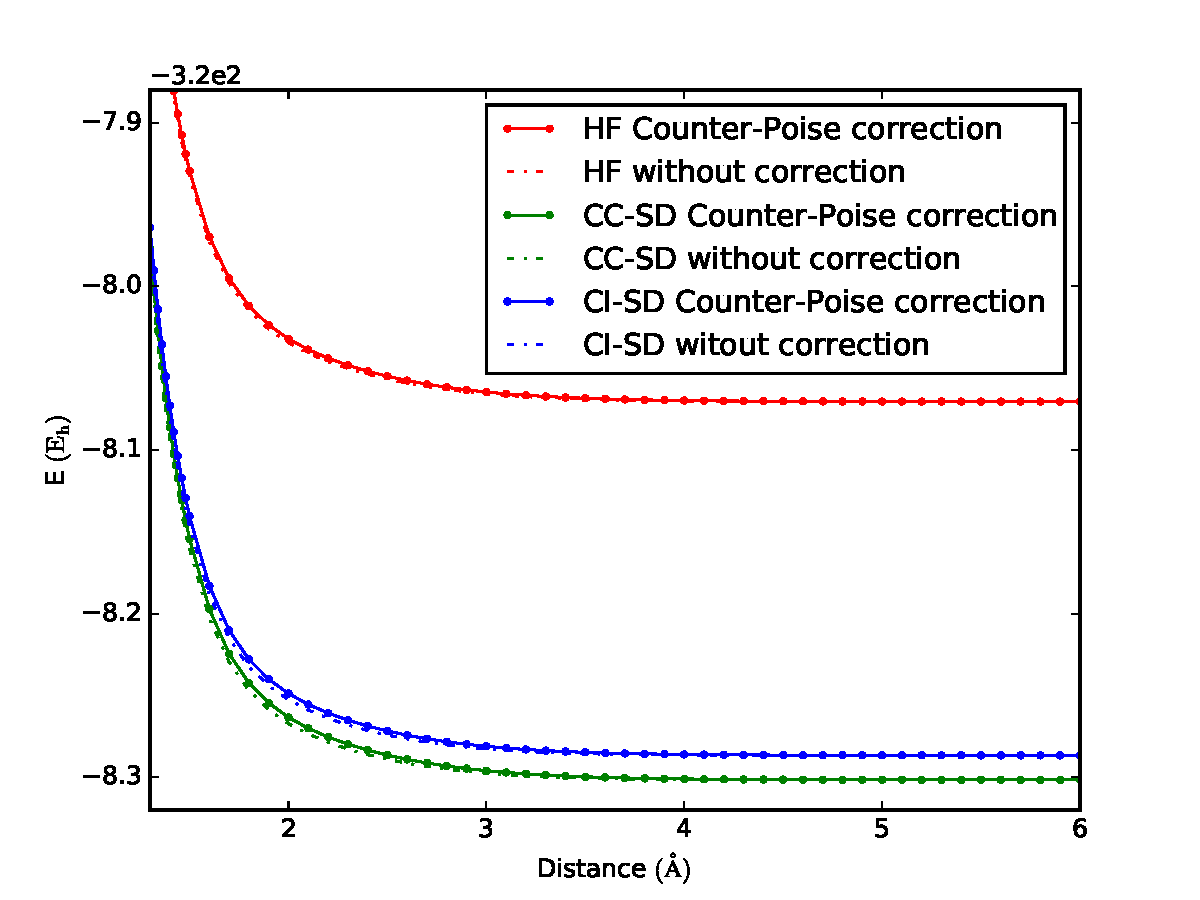
\includegraphics[width=0.47\textwidth]{./img/plots/bsse.pdf}
    \caption{Energy curve with and without the correction of BSSE.}
\label{BSSE}
\end{wrapfigure}

With the information (plotted in the Figure \ref{BSSE}), we can aim that even if
we consider or not these correction, the energy is basically the same. However
this energy difference is computable and appreciable, in the case where we are,
a small system, the correction is not time computing prohibitive, then is also
a good over-correction for better results.

Since we already have the alone energy atoms and the values for the system but so
far away, we can see the Size Consistence of the methods that we already study.
At HF theory level we have the same energy at the whole system at 100 $\AA$ and
in the addition of the two atoms computed separately. For CC-SD the same and finally
for CI-SD we have a difference of 0.01 $E\mathrm{_h}$. making sense,
since we know CI-SD is not Size Consistent, while the other two methods are.

\section{\textbf{Final Remarks}}

In this work we studied the Sapporo-DZP basis set and also -TZP \& -QZP, where
these family of basis set was studied in some others different ways, as for
example the relativistic effects.

Where was developed all-electron relativistic segmented-type basis set for
the 15 lanthanide atoms La trough Lu as member of Sapporo-$n$ZP ($n$ =
D, T, Q), which efficiently incorporate the correlation among electrons in the
valence and core shells as well as the relativistic effect.\cite{Sekiya2012}

Extending the study for all-electron relativistic segmented for the s-,
d-, and p-block atoms in the sixth period as a member of the
Sapporo-DKH3-$n$ZP ($n$ = D, T, Q). That to use in molecular program
packages such as Gaussian, Gamess, Molpro, Molcas, Turbomole, Dirac,
Nwche and Alchemy2.\cite{Noro2013}

Also was found that the x2c-SV(P)all bases yield much smaller errors than
DKH-DZP bases, which are of similar size; x2c-TZVPal and Sapporo-DZP are similar
to each other concerning both size errors \cite{Pollak2017}.

Not only relativistic studies was developed. Moreover, was studied already all
electrons non-relativistic until Xe atom \cite{Noro2012}. Even was already
studied the BSSE for alkali and alkali-earth metal atoms \cite{Noro2008}, and
atoms from K to Xe \cite{Noro2009}. These last two papers has an accuracy with
our work, since they aim that the correction around BSSE change their
calculations is around 0.01 $\mathrm{eV}$ for $D_0$, 0.01 $\AA$ for equilibrium
distances at $r_e$ and values near to 1 and 3 $\mathrm{cm}^{-1}$ for
$\omega_e$.


\section{\textbf{Supplementary Information}}\label{toomuchinformaiton}

The unit for distance is $\AA$, and for the energy in all cases is
$E\mathrm{_h}$.

% Table generated by Excel2LaTeX from sheet 'raw_data_dzp'
{\renewcommand{\baselinestretch}{.5}
\scriptsize{
\begin{longtable}{p{.20\textwidth} p{.20\textwidth} p{.20\textwidth} p{.20\textwidth}}%[htbp]
%  \centering
%    \begin{tabular}{rrrr}
%    \multicolumn{1}{l}{distance} & \multicolumn{1}{l}{hf} & \multicolumn{1}{l}{cc} & \multicolumn{1}{l}{ci} \\
    distance & HF & CC-SD & CI-SD \\
    0.50  & -315.78295858 & -315.92849684 & -315.92227849 \\
    0.52  & -317.02298268 & -317.16794513 & -317.16187962 \\
    0.54  & -318.08661556 & -318.23137257 & -318.22539742 \\
    0.56  & -319.00128270 & -319.14616707 & -319.14022651 \\
    0.58  & -319.78990025 & -319.93521469 & -319.92925985 \\
    0.60  & -320.47167797 & -320.61770586 & -320.61169402 \\
    0.62  & -321.06277663 & -321.20980063 & -321.20369276 \\
    0.64  & -321.57686402 & -321.72520375 & -321.71895893 \\
    0.66  & -322.02561922 & -322.17572368 & -322.16928382 \\
    0.68  & -322.41927766 & -322.57200544 & -322.56524031 \\
    0.70  & -322.76749366 & -322.92518902 & -322.91762782 \\
    0.72  & -323.08151923 & -323.25279858 & -323.24213343 \\
    0.74  & -323.37960200 & -323.58940256 & -323.56799210 \\
    0.76  & -323.68614876 & -323.92531226 & -323.90793459 \\
    0.78  & -324.22198341 & -324.45692459 & -324.44070893 \\
    0.80  & -324.58588494 & -324.81221061 & -324.79782671 \\
    0.82  & -324.92062133 & -325.14251035 & -325.12898319 \\
    0.84  & -325.22538684 & -325.44483497 & -325.43175055 \\
    0.86  & -325.50145430 & -325.71948183 & -325.70665155 \\
    0.88  & -325.75083410 & -325.96801648 & -325.95534210 \\
    0.90  & -325.97574587 & -326.19243508 & -326.17985890 \\
    0.92  & -326.17839818 & -326.39482287 & -326.38230766 \\
    0.94  & -326.36089316 & -326.57720853 & -326.56472854 \\
    0.96  & -326.52518652 & -326.74150142 & -326.72903796 \\
    0.98  & -326.67307414 & -326.88946692 & -326.87700586 \\
    1.00  & -326.80619202 & -327.02272027 & -327.01025063 \\
    1.02  & -326.92602283 & -327.14272972 & -327.13024279 \\
    1.04  & -327.03390583 & -327.25082442 & -327.23831313 \\
    1.06  & -327.13104806 & -327.34820431 & -327.33566286 \\
    1.08  & -327.21853590 & -327.43595094 & -327.42337442 \\
    1.10  & -327.29734627 & -327.51503806 & -327.50242232 \\
    1.12  & -327.36835718 & -327.58634192 & -327.57368332 \\
    1.14  & -327.43235753 & -327.65065074 & -327.63794601 \\
    1.16  & -327.49005601 & -327.70867340 & -327.69591959 \\
    1.18  & -327.54208913 & -327.76104740 & -327.74824170 \\
    1.20  & -327.58902853 & -327.80834590 & -327.79548563 \\
    1.22  & -327.63138747 & -327.85108411 & -327.83816663 \\
    1.24  & -327.66962673 & -327.88972494 & -327.87674766 \\
    1.26  & -327.70415986 & -327.92468413 & -327.91164444 \\
    1.28  & -327.73535800 & -327.95633472 & -327.94323006 \\
    1.30  & -327.76355417 & -327.98501115 & -327.97183901 \\
    1.32  & -327.78904720 & -328.01101291 & -327.99777089 \\
    1.34  & -327.81210529 & -328.03460779 & -328.02129371 \\
    1.36  & -327.83296922 & -328.05603492 & -328.04264688 \\
    1.38  & -327.85185525 & -328.07550751 & -328.06204403 \\
    1.40  & -327.86895778 & -328.09321544 & -328.07967554 \\
    1.42  & -327.88445169 & -328.10932773 & -328.09571105 \\
    1.44  & -327.89849442 & -328.12399484 & -328.11030171 \\
    1.46  & -327.91122787 & -328.13735097 & -328.12358244 \\
    1.48  & -327.92278005 & -328.14951617 & -328.13567403 \\
    1.50  & -327.93326651 & -328.16059829 & -328.14668501 \\
    1.60  & -327.97303608 & -328.20288375 & -328.18866916 \\
    1.70  & -327.99820634 & -328.22962492 & -328.21521242 \\
    1.80  & -328.01474232 & -328.24697731 & -328.23244932 \\
    1.90  & -328.02615944 & -328.25876051 & -328.24416714 \\
    2.00  & -328.03448666 & -328.26721194 & -328.25257895 \\
    2.10  & -328.04087827 & -328.27360270 & -328.25894077 \\
    2.20  & -328.04598674 & -328.27864823 & -328.26395983 \\
    2.30  & -328.05018347 & -328.28275398 & -328.26803794 \\
    2.40  & -328.05368712 & -328.28615674 & -328.27141102 \\
    2.50  & -328.05663521 & -328.28900293 & -328.27422616 \\
    2.60  & -328.05912145 & -328.29139001 & -328.27658206 \\
    2.70  & -328.06121460 & -328.29338786 & -328.27854984 \\
    2.80  & -328.06296845 & -328.29505036 & -328.28018439 \\
    2.90  & -328.06442779 & -328.29642226 & -328.28153108 \\
    3.00  & -328.06563199 & -328.29754313 & -328.28262980 \\
    3.10  & -328.06661698 & -328.29844930 & -328.28351698 \\
    3.20  & -328.06741590 & -328.29917438 & -328.28422614 \\
    3.30  & -328.06805897 & -328.29974899 & -328.28478776 \\
    3.40  & -328.06857321 & -328.30020041 & -328.28522888 \\
    3.50  & -328.06898216 & -328.30055225 & -328.28557286 \\
    3.60  & -328.06930591 & -328.30082446 & -328.28583936 \\
    3.70  & -328.06956123 & -328.30103358 & -328.28604461 \\
    3.80  & -328.06976190 & -328.30119305 & -328.28620175 \\
    3.90  & -328.06991915 & -328.30131372 & -328.28632132 \\
    4.00  & -328.07004199 & -328.30140422 & -328.28641166 \\
    4.10  & -328.07013763 & -328.30147139 & -328.28647935 \\
    4.20  & -328.07021182 & -328.30152061 & -328.28652955 \\
    4.30  & -328.07026913 & -328.30155608 & -328.28656629 \\
    4.40  & -328.07031316 & -328.30158111 & -328.28659271 \\
    4.50  & -328.07034677 & -328.30159826 & -328.28661127 \\
    4.60  & -328.07037225 & -328.30160951 & -328.28662390 \\
    4.70  & -328.07039139 & -328.30161641 & -328.28663207 \\
    4.80  & -328.07040561 & -328.30162015 & -328.28663695 \\
    4.90  & -328.07041604 & -328.30162165 & -328.28663945 \\
    5.00  & -328.07042359 & -328.30162159 & -328.28664026 \\
    5.10  & -328.07042894 & -328.30162051 & -328.28663991 \\
    5.20  & -328.07043265 & -328.30161880 & -328.28663881 \\
    5.30  & -328.07043516 & -328.30161674 & -328.28663725 \\
    5.40  & -328.07043678 & -328.30161454 & -328.28663546 \\
    5.50  & -328.07043778 & -328.30161235 & -328.28663358 \\
    5.60  & -328.07043834 & -328.30161024 & -328.28663174 \\
    5.70  & -328.07043860 & -328.30160829 & -328.28662998 \\
    5.80  & -328.07043866 & -328.30160652 & -328.28662837 \\
    5.90  & -328.07043861 & -328.30160494 & -328.28662691 \\
    6.00  & -328.07043849 & -328.30160355 & -328.28662561 \\
    6.10  & -328.07043833 & -328.30160235 & -328.28662447 \\
    6.20  & -328.07043816 & -328.30160132 & -328.28662348 \\
    6.30  & -328.07043800 & -328.30160044 & -328.28662262 \\
    6.40  & -328.07043784 & -328.30159969 & -328.28662189 \\
    6.50  & -328.07043771 & -328.30159905 & -328.28662126 \\
    7.50  & -328.07043714 & -328.30159623 & -328.28661839 \\
    8.50  & -328.07043709 & -328.30159557 & -328.28661765 \\
    9.50  & -328.07043709 & -328.30159530 & -328.28661735 \\
    10.50 & -328.07043709 & -328.30159518 & -328.28661722 \\
    11.50 & -328.07043709 & -328.30159512 & -328.28661714 \\
    12.50 & -328.07043709 & -328.30159508 & -328.28661711 \\
    13.50 & -328.07043709 & -328.30159506 & -328.28661709 \\
    14.50 & -328.07043709 & -328.30159505 & -328.28661707 \\
    15.50 & -328.07043709 & -328.30159504 & -328.28661706 \\
    16.50 & -328.07043709 & -328.30159504 & -328.28661706 \\
    17.50 & -328.07043709 & -328.30159504 & -328.28661706 \\
    18.50 & -328.07043709 & -328.30159503 & -328.28661705 \\
    19.50 & -328.07043709 & -328.30159503 & -328.28661705 \\
    20.50 & -328.07043709 & -328.30159503 & -328.28661705 \\
    21.50 & -328.07043709 & -328.30159503 & -328.28661705 \\
    22.50 & -328.07043709 & -328.30159503 & -328.28661705 \\
    23.50 & -328.07043709 & -328.30159503 & -328.28661705 \\
    24.50 & -328.07043709 & -328.30159503 & -328.28661705 \\
    25.50 & -328.07043709 & -328.30159503 & -328.28661705 \\
    26.50 & -328.07043709 & -328.30159503 & -328.28661705 \\
    27.50 & -328.07043709 & -328.30159503 & -328.28661705 \\
    28.50 & -328.07043709 & -328.30159503 & -328.28661705 \\
    29.50 & -328.07043709 & -328.30159503 & -328.28661705 \\
    30.50 & -328.07043709 & -328.30159503 & -328.28661705 \\
    31.50 & -328.07043709 & -328.30159503 & -328.28661705 \\
    32.50 & -328.07043709 & -328.30159503 & -328.28661705 \\
    33.50 & -328.07043709 & -328.30159503 & -328.28661705 \\
    34.50 & -328.07043709 & -328.30159503 & -328.28661705 \\
    35.50 & -328.07043709 & -328.30159503 & -328.28661705 \\
    36.50 & -328.07043709 & -328.30159503 & -328.28661705 \\
    37.50 & -328.07043709 & -328.30159503 & -328.28661705 \\
    38.50 & -328.07043709 & -328.30159503 & -328.28661705 \\
    39.50 & -328.07043709 & -328.30159503 & -328.28661705 \\
    40.50 & -328.07043709 & -328.30159503 & -328.28661705 \\
    41.50 & -328.07043709 & -328.30159503 & -328.28661705 \\
    42.50 & -328.07043709 & -328.30159503 & -328.28661705 \\
    43.50 & -328.07043709 & -328.30159503 & -328.28661705 \\
    44.50 & -328.07043709 & -328.30159503 & -328.28661705 \\
    45.50 & -328.07043709 & -328.30159503 & -328.28661705 \\
    46.50 & -328.07043709 & -328.30159503 & -328.28661705 \\
    47.50 & -328.07043709 & -328.30159503 & -328.28661705 \\
    48.50 & -328.07043709 & -328.30159503 & -328.28661705 \\
    49.50 & -328.07043709 & -328.30159503 & -328.28661705 \\
    50.50 & -328.07043709 & -328.30159503 & -328.28661705 \\
    51.50 & -328.07043709 & -328.30159503 & -328.28661705 \\
    52.50 & -328.07043709 & -328.30159503 & -328.28661705 \\
    53.50 & -328.07043709 & -328.30159503 & -328.28661705 \\
    54.50 & -328.07043709 & -328.30159503 & -328.28661705 \\
    55.50 & -328.07043709 & -328.30159503 & -328.28661705 \\
    56.50 & -328.07043709 & -328.30159503 & -328.28661705 \\
    100.00 & -328.07043709 & -328.30159503 & -328.28661705 \\
%    \end{tabular}%
\end{longtable}%


\normalsize
